\paragraph{Klassifisering av forsterkere} \mbox{} \\
Forksjellige parametre definerer egenskapene til en forsterker.
Avhengig av hvilken karakteristikk man ser på kan forsterkerne klassifiseres.
\\
\begin{itemize}
\item Lav og høy frekvens
\item Avstemt og uavstemt
\item Smalbånd og bredbånd
\end{itemize}

I de følgende seksjonene skal vi se på effektforsterkere og hvordan de deles inn
etter hvordan transistorens arbeidspunkt er plassert på lastlinja.
\\
Effektforsterkere har en virkningsgrad som sier noe om effekten ut
i forhold til effekten inn.
$$\eta = \frac{P_L}{P_{CC}} $$
Hvor \\
 $P_L$ = Effekt avgitt fra lasten og \\
$P_{CC}$ = Effekt tilført fra CC.

\subsubsection{Klasse A}
Arbeidspunktet ligger midt på lastlinja.
Altså i det aktive området.
\\
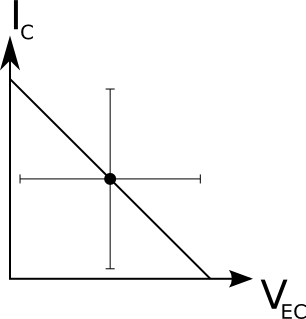
\includegraphics[width=0.5\textwidth]{./img/typeALastlinje}
\\\\
Effektforsterker klasse A (emitterfølger)
\\
\begin{circuitikz} \draw
(4,2) node[npn] (npn) {}
      (npn.base) node[anchor=east] {}
      (npn.collector) node[anchor=south] {}
      (npn.emitter) node[anchor=north] {}

(0,2) node[label=$V_{inn}$] {}
      to[C, o-] (2,2)
      -- (npn.base)
(2,2) to[R, l=$R_1$] (2,4)
      -- (4,4)
      -- (npn.collector)
(2,2) to[R, l=$R_2$] (2,-1)
(npn.emitter) to[R, l=$R_E$] (4,-1)
(4,1) to[short, -o] (6,1)
      node[label=$V_{ut}$] {}
(4,-1) -- (0,-1)
      node[ground] {}
      ;
\end{circuitikz}
\\\\
TypeA effektforsterkere har lav virkningsgrad. f.eks $\eta = 25\%$.
Denne klassen trekker strøm når det ikke er tilført signal.


\subsubsection{Klasse B}
Arbeidsområdet er på grensa mellom aktiv og cutoff.
\\
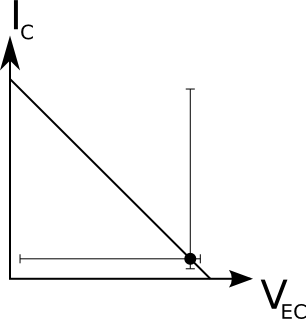
\includegraphics[width=0.5\textwidth]{./img/typeBLastlinje}
\\
I en klasse B emitterfølger blir det en effektforsterkning som kun
virker på halvperioder.
Output signalet tar ikke med negativt input signal.
\\\\
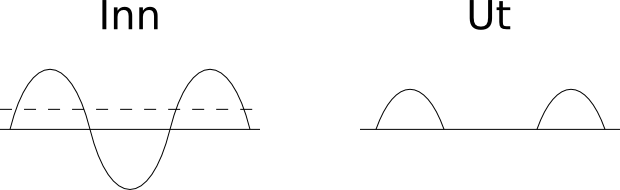
\includegraphics[width=0.67\textwidth]{./img/klasseBSignal}
\\\\
En slik forsterker ser slik ut
\\
\begin{circuitikz} \draw
(4,3) node[npn] (npn) {}
      (npn.base) node[anchor=east] {}
      (npn.collector) node[anchor=south] {}
      (npn.emitter) node[anchor=north] {}

(0,0) node[ground] {}
      to[vsourcesin, l=$V_{inn}$] (0,3)
      -- (npn.base)
(npn.collector) to[short, -o, l=$V_{CC}$] (4,4)
(npn.emitter) -- (4,2)
      to[R, l=$R_E$] (4,0)
      node[ground] {}
(4,2) to[short, -o, l=$V_{ut}$] (5,2)
      ;
\end{circuitikz}
\\\\
Det finnes også \emph{Push-Pull} klasse B forsterkere.
De bruker både npn og pnp og fanger både positive og negative signaler, men
med \emph{crossover} forvrengning.
\\\\
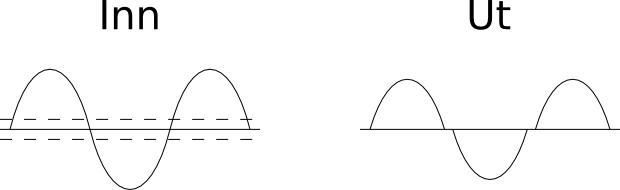
\includegraphics[width=0.67\textwidth]{./img/crossover}


\subsubsection{Klasse AB}
TODO


\subsubsection{Klasse C}
TODO


\subsubsection{Klasse D}
TODO

